\subsection{Departamento}

  \paragraph{}Se procede a crear el departamento al que pertenece el asesor,
  en este caso, \textit{Biología celular}. Para ello, se realizará
  la creación de un departamento, tal y como se describió en el capítulo
  \ref{addDepartamento}, \textit{Añadir departamento}.

  \paragraph{}Una vez que aparezca el formulario de creación, se debe introducir
  el nombre del departamento, con lo que la pantalla quedaría tal
  y como refleja la figura \ref{ejemploAddDepartamento}.

  \begin{figure}[!ht]
    \begin{center}
      \fbox{
      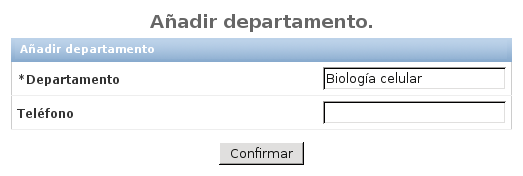
\includegraphics[scale=0.55]{5.Ejemplos_Practicos/5.3.IntroduccionDatos/5.3.5.Departamento/add_departamento.png}
      }
      \caption{Creación de \textit{Departamento} de ejemplo.}
      \label{ejemploAddDepartamento}
    \end{center}
  \end{figure}

  \paragraph{}Una vez rellenado el formulario, se pulsará el botón
  \textit{Confirmar}, el cual se puede ver en la figura
  \ref{capturaBotonConfirmar}. Si el formulario rellenado es válido, y no tiene
  errores, se creará el nuevo elemento en el sistema. En caso de contener
  información no válida, un mensaje de error aparecerá indicando los campos
  del formulario que no han pasado la validación, los cuales habrá que modificar
  para introducir correctamente el elemento en el sistema.
